\documentclass[cjk]{beamer}
\usepackage{CJK}
\usepackage{amsmath}
\usepackage{graphicx}
\usepackage{float}
\usepackage{fancyhdr}
\usepackage{algorithm}
\usepackage{algpseudocode}

\usetheme{CopenHagen}
\usecolortheme{seagull}
\begin{document}
\begin{CJK*}{UTF8}{gbsn}
\title{streaming lib.}
\author{金奕成$\ $黄道吉$\ $杨天正}
\institute{算分29班}
\date{\today}

\begin{frame}
  \titlepage
\end{frame}

\begin{frame}
  \frametitle{content}
  \tableofcontents
\end{frame}

\section{introduction}
  \begin{frame}
    \frametitle{streaming algorithm}
    \begin{itemize}
      \item 流算法(streaming algorithm)在网络流, 数据库和文本处理当中有比较重要的应用
      \item 两种重要的方面是hashing和sketch, 我们将完成这两个部分的一些基本算法, 并封装成库.
    \end{itemize}
  \end{frame}

  \begin{frame}
    \frametitle{references}
    目前主要参考以下几篇论文
    \begin{itemize}
      \item Cormode, Graham. “Sketch Techniques for Approximate Query Processing.” (2010).
      \item Charikara, Moses and Martin Farach-Coltonc. “Finding frequent items in data streams.” (2003).
      \item Muthukrishnan, S.. “Data streams: algorithms and applications.” SODA (2003).
    \end{itemize}
  \end{frame}

\section{contents}
  \subsection{Frequency based sketch}
    \begin{frame}
      \frametitle{Frequency based sketch}
      \begin{itemize}
        \item Count Sketch, Count-Min Sketch是两种常用的基于频率的sketch
        \item 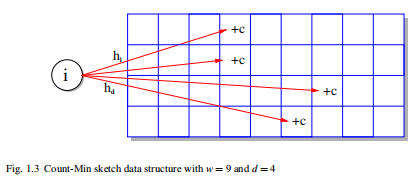
\includegraphics[scale = 0.5]{1.png}
        \item 此外也有AMS$\ $sketch之类的sketch.
      \end{itemize}
    \end{frame}

  \subsection{Distinct Count Estimation}
    \begin{frame}
      \frametitle{Distinct Count Estimation}
      \begin{itemize}
        \item 主要有Flajolet-Martin Sketch, $k$ Minimum Value estimator之类的算法
        \item 基于hash还可以将前面的算法做到更好
        \item 支持一些基础的skipping, sampling技术.
      \end{itemize}
    \end{frame}

\section{goals}
  \begin{frame}
    \frametitle{goals}
    我们的目标是实现
    \begin{itemize}
      \item 主流, 常见的一些sketch, 及其变体
      \item 实现必要的hash函数支持
      \item 提供测试程序
      \item 提供对多种数据的支持(五元组)
    \end{itemize}
  \end{frame}

\end{CJK*}
\end{document}
